\documentclass[12pt,letterpaper]{article}
\usepackage{natbib}

%Packages
\usepackage{xcolor}
\usepackage{color,soul}
\usepackage{pdflscape}
\usepackage{fixltx2e}
\usepackage{textcomp}
\usepackage{fullpage}
\usepackage{float}
\usepackage{latexsym}
\usepackage{url}
\usepackage{epsfig}
\usepackage{graphicx}
\usepackage{amssymb}
\usepackage{amsmath}
\usepackage{bm}
\usepackage{array}
\usepackage[version=3]{mhchem}
\usepackage{ifthen}
\usepackage{caption}
\usepackage{hyperref}
\usepackage{amsthm}
\usepackage{amstext}
\usepackage{enumerate}
\usepackage[osf]{mathpazo}
\usepackage{dcolumn}
\usepackage{lineno}
\usepackage{dcolumn}
\usepackage{hyphenat}
\usepackage[T1]{fontenc}
\usepackage{textcomp}
\newcolumntype{d}[1]{D{.}{.}{#1}}

\pagenumbering{arabic}


%Pagination style and stuff
\linespread{2}
\raggedright
\setlength{\parindent}{0.5in}
\setcounter{secnumdepth}{0} 
\renewcommand{\section}[1]{%
\bigskip
\begin{center}
\begin{Large}
\normalfont\scshape #1
\medskip
\end{Large}
\end{center}}
\renewcommand{\subsection}[1]{%
\bigskip
\begin{center}
\begin{large}
\normalfont\itshape #1
\end{large}
\end{center}}
\renewcommand{\subsubsection}[1]{%
\vspace{2ex}
\noindent
\textit{#1.}---}
\renewcommand{\tableofcontents}{}
%\bibpunct{(}{)}{;}{a}{}{,}

%---------------------------------------------
%
%       START
%
%---------------------------------------------

\begin{document}

%Running head
\begin{flushright}
Version dated: \today
\end{flushright}
\bigskip
\noindent RH: pest practices for disparity analysis.

\bigskip
\medskip
\begin{center}

\noindent{\Large \bf Analysing disparity in morphology data: best practice and future directions} 

\bigskip

\noindent {\normalsize \sc Thomas Guillerme$^{1,*,+}$, Natalie Cooper$^{2,+}$, Stephen Brusatte$^3$, Katie Davis$^4$, Andrew Jackson$^5$, Sylvain Gerber$^6$, Anjali Goswami$^2$, Kevin Healy$^7$, Melanie Hopkins$^8$, Graeme Lloyd$^9$, Joseph O'Reilly$^{10}$, Abi Pate$^{10}$, Emilie Rayfield$^{10}$, Erin Saupe$^{11}$, Emma Sherratt$^{12}$, Graham Slater$^{13}$, Gavin H Thomas$^{14}$ and Philip Donoghue$^{10,+}$}\\


\noindent {\small \it 
$^1$School of Biological Sciences, University of Queensland, St. Lucia, Queensland, Australia.\\ 
$^2$Department of Life Sciences, Natural History Museum, London, Cromwell Road, London, SW7 5BD, UK.\\ 
$^{10}$Bristol}
\end{center}
\medskip
\noindent{+ These authors contributed equally to the manuscript.}
\noindent{*\bf Corresponding author.} \textit{guillert@tcd.ie}\\  
\vspace{1in}

%Line numbering
\modulolinenumbers[1]
\linenumbers


%---------------------------------------------
%
%       ABSTRACT
%
%---------------------------------------------

\newpage
\begin{abstract}

Variation in organisms' shape, ecology or behaviour is often more discrete rather than continuous.
One way to study this variation was pioneered in the 1990s by looking at the disparity of morphologies in the Cambrian.
Morphological disparity analysis - a term encompassing both the patterns and process of morphological evolution through time - became rapidly popular and lead to numerous publications in the last two decades.

Here, we suggest that this diversification of disparity analysis lead to two contrasted effects:
(1) the great diversity of methodological approaches to study disparity makes it sometimes hard to understand all caveats and pitfalls of such analysis - a problem that can lead to major misinterpretation of disparity patterns - and;
(2) in essence, disparity is a pattern of variation meaning that disparity analysis can be expanded beyond the study of morphology.

In this review, we propose a set of non-prescriptive guidelines that will help researchers to think about specific disparity analysis designs, with their caveats and their advantages.
Furthermore, we highlight potential avenues of expansion of disparity analysis both in terms of improving the existing methods for studying morphological disparity and in terms of expanding disparity analysis beyond morphology.

\end{abstract}

\noindent (Keywords: disparity)\\

\vspace{1.5in}

\newpage 

%---------------------------------------------
%
%       INTRODUCTION
%
%---------------------------------------------
\section{Introduction}

Variation in the shape, form and function of organisms often follows discrete patterns rather than continuous gradients.
These patterns can be pictured as multidimensional spaces encompassing all the possible forms an organism can take, and where each individual region of this space is the result of a discrete combination of many variables.
One commonly used approach to analyse these discrete patterns, and to understand the processes that lead to them, is to analyse the disparity of the morphological characteristics of the group, often referred to as ``morphological disparity analysis''.
% The multidimensional space for mammalian carnivores, for example, encompasses all combinations of the traits of the order Carnivora, along with the ecological, life history and behavioural variables characteristic of meat eating mammals.
% Each individual carnivore species occupies a discrete region of this space related to its values for these traits.

In the seminal disparity papers from the late 1980s, disparity was used to investigate body plan evolution after the Cambrian explosion (REF)[Runnegar 1987, Gould, Foote, Webb, etc.].
Early disparity analyses focused on broad questions such as: How does diversity evolve? Are some body types more common than others? Can shape evolve in all ``directions'' (of the multidimensional space)?
Since the 1980s, a great deal of literature from a range of sub-fields in biology, and an equally large number of methods, have used the term ``disparity''.
Disparity analysis has been used to tackle a vast array of questions, for example in evo-devo (i.e. developmental constraints [CITE]; relationships between form and function [CITE]; evolution functional traits [CITE]; and scaling from micro- to macro-level processes [CITE]), in ecology and palaeoecology (i.e. intra-specific competition [CITE], niche occupancy[CITE]; speciation[CITE]; competition [CITE]; and macroecology/disparity in space[CITE]), and macroevolution (i.e. responses to extinction and extinction selectivity [CITE]; intra-specific competitive replacements [CITE]; and tempo and mode of evolution [CITE]).

The initial informal definition of disparity was ``multidimensional morphological dissimilarity at a macroevolutionary scale'' (REFS).
Currently, however, there is no consensus on whether we should restrict use of the term disparity to this initial definition, or whether it should be used as a broader umbrella term for studies of multivariate variation (REF Katie et al's paper somewhere here). 
Here we use a broader definition and suggest that disparity is a pattern of variation.
Throughout this review, we aim to highlight the diversity of ``disparity'' analyses and how they can aid our understanding of the structure of biodiversity.

% \subsection{What \textit{is} disparity?} %TG: maybe useful for box or paraphrapsing summaries.
% What \textit{is} disparity? In the seminal disparity papers from the late 80s, disparity was used in analyses of body plan evolution after the Cambrian explosion (REF).
% The initial informal definition of disparity was, therefore, ``multidimensional morphological dissimilarity at a macroevolutionary scale''.
% Currently, there is no consensus on whether we should restrict use of the term disparity to this initial definition, or whether it should be used as a broader umbrella term for studies of multivariate variation. 
% There is also debate about whether disparity refers to a pattern, a process that generates the pattern, or both. 
% Even if disparity only describes patterns of variation, the scientific questions of disparity analyses generally use these patterns as a proxy for explaining the biological processes underlying them.
% The original Cambrian explosion papers, for example, use disparity to describe both the pattern of high dissimilarity in body plans among groups, and the process of explosive radiation that generated them (as championed by Gould; REF). 

% Restricting disparity to its original definition can be advantageous for advances in this field but broadening it allows more interdisciplinary discussion.
% In recent years, disparity has been used to investigate ecological processes, disconnected from evolution (e.g. function [CITE], community structure[CITE], competition[CITE]).
% Thus studying disparity could not only inform us on macroevolutionary patterns and processes but also something about environments and ecosystem functioning (with the advantages of easily allowing palaeocological and palaeoenvironemental perspectives).

\section{Best practices for disparity analysis}

This diversity (and disparity) of methods to analysis disparity provides biologists with a powerful and comprehensive toolkit for understanding the evolution of biological diversity.
However, as with any great power, it comes with great responsibility. 
With the expansion of methodological approaches in the last decade, we identify three main issues that could reduce the power of disparity analyses if they are not tackled.
First, many recent studies have lost focus; they are no longer hypothesis-driven, instead they are undertaken to characterise biological variation for its own sake.
Second, even where there is a clear question being explored, the data being used for disparity analyses is inappropriate and often driven by the availability of large datasets rather than the question being asked.
Third, the methods being used to analyse these datasets may not always be appropriate for the question and/or data at hand.
Here we deal with some of these issues and present best practice guidelines to allow researchers to optimise their disparity analysis.

\section{What is the question?}
Why perform a disparity analysis?
This seems like it should be obvious, but we stress its crucial importance.
The last decade has seen a vast array of new methods being published and implemented in freely available software, making disparity analyses easy to perform \citep{bouxin2005ginkgo,oksanen2007vegan,geiger2008,zelditch2012geometric,adams2013geomorph,Claddis,dispRityv02,adams2017geometric}.
However, this (consciously or not) pushes authors towards performing disparity analyses simply because of their ease of implementation, rather than stemming from a question driven approach.
Before rushing into a disparity analysis, one should consider some basic caveats.
For example, one major thing to consider is circularity: if the aim is to explore the variation in a dataset, disparity analysis is perfectly valid.
However, if this exploratory analysis reveals distinct groups, it would be circular to then test for differences among those groups as if this had been the hypothesis all along [CITE stats 1.0].
This can easily be avoided by using a subset of the data for preliminary data exploration, and then using the full dataset to test for differences among any groups that emerge.
Clearly framing questions and their null expectations will help in designing better disparity analyses.

\section{Collect the appropriate data}
Once one has a clear question, it is important to collect the appropriate data for that question to avoid some major caveats.
For example, if a study focuses on the ecological adaptive radiation of a group, ecological traits are crucial and should be preferred over other kinds of traits, such as those used for species delimitation.
Tangentially, more data are not necessarily better, especially when the data were originally collected for different questions (e.g. cladistic data - see below).

\subsection{Data types}
Morphological disparity analysis can be based on three main types of data:
\begin{enumerate}
    \item discrete data that can either describe a feature (often referred to as ``cladistic''; e.g. the presence or absence of legs, the colour of a tail, etc. [CITE]) or count the number of features (e.g. number of digits, etc. [CITE]);
    \item continuous data that can be either simple measurements (e.g. body length, etc. [CITE]) or more abstracted measures (e.g. geometric morphometrics, mathematical contour description, etc. [CITE]);
    \item any mixture of discrete and continuous data (e.g. ratios [CITE]).
\end{enumerate}
None of these types of data are fundamentally better but each will be more appropriate for specific questions.
For example, when investigating variation within bat wing shapes, both homologous landmarks (for geometric morphometric analysis) or continuous measurements of bones may be appropriate.
On the other hand, if the question focuses on the convergence between bat and bird wings, the homology of the traits to measure is more complex to define and the outline shape of the wings might more readily answer the question.
This again illustrates the importance of framing the question.
In the above example, if the question is whether the aerodynamic properties of wings vary within bats or between bats and birds, the traits collected should reflect these aerodynamic properties (e.g. wingspan, aspect ratio, etc.).
Conversely if the question focuses on phylogenetic convergence aspects between different types of species with active flight, it might be more pertinent to use evolutionary traits that may have facilitated flight within and between both groups (e.g. digit length, integumentary system, etc.).

\subsection{How much data should be collected?}
Regardless of the type of data, another important consideration is how much data to collect, in terms of numbers of specimens and traits.
\begin{itemize}
    \item \textit{Taxonomic scope.}
    Morphological disparity has been studied at both inter-[CITE] and intra-specific levels [CITE].
    Taxonomic scope will depend on the question being investigated, and what type of variation is being analysed.
    For example, when studying skull shape plasticity in canids, it is essential to include intra-specific variation to capture the full variety of skull shapes, particularly that seen in domestic dogs (CITE).
    Conversely, if a study focuses on canid skull variation through time, interspecific data is most appropriate.
    % intra-specific variation will not have major impact (up until the Holocene). %http://www.journals.uchicago.edu/doi/abs/10.1086/650372
    \item \textit{Sample size.}
    It is important to ensure that the data is collected in a way that will not bias subsequent statistical analysis.
    For example, if the aim is to compare disparity among groups, one should collect, where possible, a similar amount of data for each group.
    When this is not possible (e.g. for palaeontological data), one should use statistical approaches to correct or assess biases due to data collection (e.g. rarefaction [CITE]).
    Equally, one should ensure that enough data is available so that the methods have power to detect the patterns being tested.
    \end{itemize}

Of course in practice some of these caveats are unavoidable, especially when dealing with the vertebrate fossil record.

\subsection{Recycling data}
A common practice in morphological disparity analysis is to recycle data from other studies which can introduce additional problems.
One classic case is using ``cladistic'' data in palaeobiology.
These data are usually collected for phylogenetic analysis and are thus designed to maximise differences among taxa to recover a clear phylogenetic signal.
It can therefore artificially lead to maximised disparity among taxa [Foote - crinoids non-cladistic paper].
A relatively simple way to reduce this specific bias is to select the most pertinent characters for the question from the dataset, rather than using all of the data.
For example, in a study of the disparity of dietary niches, removing non-dietary characters is a good approach.
However, it is important to remember that there is no one-to-one mapping between form and function, and that some characters can have multiple functions (e.g. limb traits can be used for both locomotion and feeding).

\subsection{Other data considerations}
There are many other considerations when choosing the appropriate data to use. 
It is essential to ensure that disparity patterns can be linked to general processes rather than being simply the reflection of idiosyncrasies in the data.
For example, are the observed differences between two groups related to factors unrelated to group designation such as sexual dimorphism?
Are the taxa/groups being compared fairly consistent and truly comparable?
In addition, data can be missing, non-overlapping, hierarchical (e.g. inapplicable), ambiguous, polymorphic or correlated [String of morpho data problems cite].
It is important to ensure that any patterns detected are not merely reflections of these features of the data.

Ultimately, data collection is often constrained by the time available, financial considerations and other unavoidable issues, however, these caveats should be kept in mind during the analyses and subsequent interpretation of the results.

\section{Use the appropriate methods} 
In the vast majority of morphological disparity analyses, the methodological approach will be multidimensional.
Multidimensional analysis can be a powerful tool for analysing complex datasets but also comes with many mathematical caveats and limitations.
The first step in any statistical analysis should be to visualise the data to understand its distribution and limitations.
Unfortunately, we can only perceive a maximum of three dimensions at the same time.
Therefore one of the main challenges in multidimensional analysis is how to reduce the number of dimensions, both for visualisation and analysis (see box \ref{box_ordination}).

\subsection{Visualising the multidimensional problem}
\label{visualisation}
It is important to remember that visual interpretations of multidimensional data can easily be misleading.
For example, it is incorrect to assume that because some groups overlap on a bivariate or three dimensional plot, that they overlap across the whole multidimensional space (especially if the space is not Euclidean).
Conversely, when two groups do not overlap on a two or three dimensional plot, this does not mean they never overlap in the multidimensional space.
Furthermore, multidimensional spaces are not necessary Euclidean.
Such non-Euclidean spaces often have non-intuitive properties, for example straight lines in some dimensions are not straight in the space and, even less intuitively, the distance between points A and B might not be equal to the distance between points B and A [CITE Sylvain].


\begin{figure}[!htbp]
\centering
   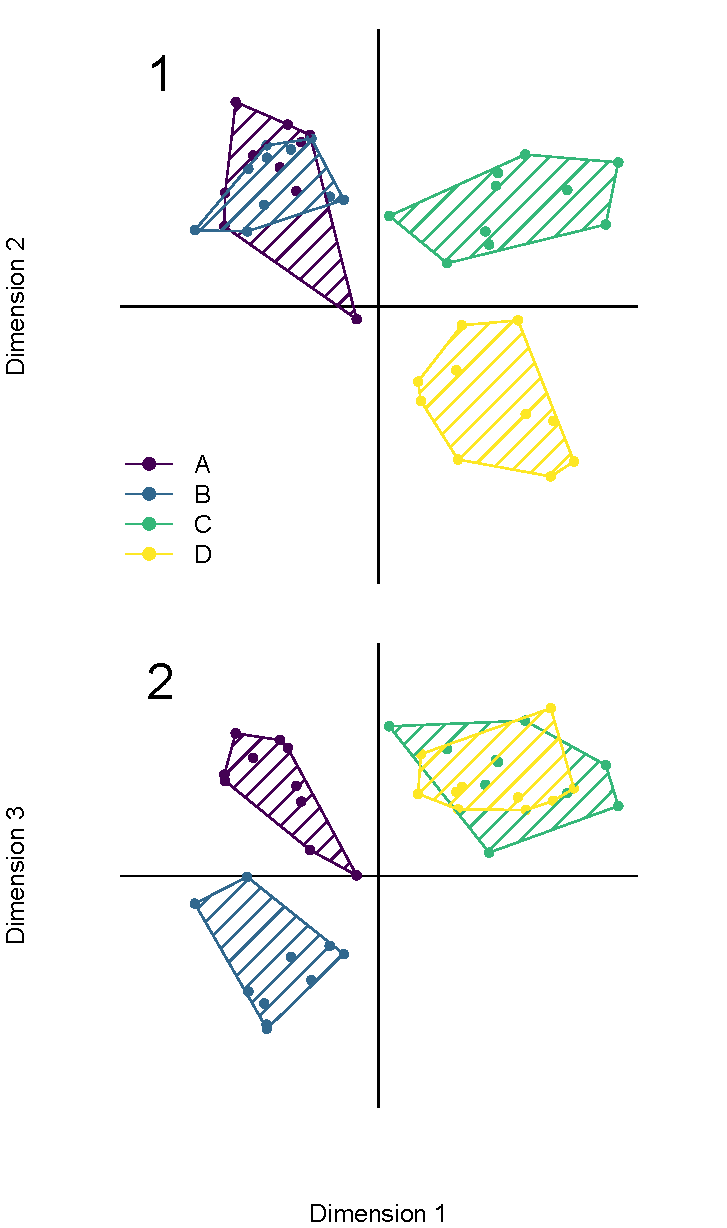
\includegraphics[width=0.5\textwidth]{Figures/dimensionsOverlap.pdf}
\caption{\small{Two groups that overlap in some dimensions do not necessary overlap in all dimensions. 
Conversely, two groups that do not overlap in some dimensions can overlap in other dimensions.
In this example for the groups A and B to truly overlap, they must overlap in all three dimensions displayed here.
Although these groups overlap in the two first dimensions (panel 1), they do not overlap in dimensions 1 and 3 thus do not overlap in the multidimensional space at all.
The inverse is of course true: if two groups don't overlap in two dimensions (D and C in panel 1), they do not overlap in the multidimensional space, even if they overlap in any other combination of dimensions (dimensions 1 and 3 in panel 2).}} 
\label{Fig:RF_results_best}
\end{figure}

It is therefore vital to be clear about what is represented in multidimensional space visualisations.
In fact, it can be easy (intentionally or not) to mislead a reader into over/under interpreting a pattern if all the key properties of the space are not present in the graph.
We suggest visualisations should include the following:
(1) the percentage of the variation explained by each axis of the plot (i.e. is the majority - or all - the variation in the data present in the plot or only a small fraction?);
(2) the scale of the axes (ideally, if the space is orthogonal, it is important to keep the same scale across the axes);
and (3) the error associated with each point, whether this is in terms of measurement error (on ordination plots for example) or some other measure of standard variation (in further analysis, e.g. disparity-through-time plots).
Finally, it is important to remember that for any dimensionality reduction of a multidimensional problem, the visual result will be at best a distortion of the measured reality, at worst, it will be misleading (see box \ref{box_ordination}).

\subsection{[Box]To ordinate or not to ordinate; that is the (multidimensional) question?}
\label{box_ordination}
Reducing the dimensionality of data through ordination can be advantageous for plotting and visualising the data, and can reveal properties of the morphospace not captured by disparity metrics (see Metrics section \ref{metrics}).
Additionally, after ordinating the data it is possible to further reduce the number of dimensions by only selecting a certain number of axes (e.g. selecting only the axes that describe up to 95\% of the variation).
In the case of geometric morphometric data, ordination is particularly useful as it conserves the mathematical properties of the data while efficiently reducing the dimensions.
This has clear advantages for interpreting the results.
For example, the axes will represent gradients of biological variation (e.g. elongation and flattening of the beak REF).

However, some caveats can arise from such transformations of the data.
For example, in the case of an ordination in a geometric morphometric data context, not using all the axes from the ordination (e.g. only the first few) can lead to misinterpretation of the results.
Furthermore, interpreting biological variation along the axes is always a \textit{post-hoc} procedure and might have little relation to the disparity question (e.g. if the first few axes represent the elongation of the beak, but the question is about wing disparity).

In many cases, ordination might not be necessary.
For example, if the disparity metric being used relies on all the data (see Metrics section \ref{metrics}) it is not necessary to calculate it on ordinated data [e.g. CITE Close].
Additionally, in some cases, reducing the dimensionality of a dataset can render its interpretation more problematic.
For example, when the analysed data is non-Euclidean (e.g. discrete morphological characters), the ordination can be problematic ([cite Melanie's future paper here]), and the resulting non-Euclidean ordinated space can be difficult to interpret ([probably cite Sylvain's here]).
This can be problematic when comparing the position of groups in the multidimensional space, as the measured distances might not be comparable.
Finally, the \textit{post-hoc} interpretation of the gradient of variation on the ordination axes can be impossible or biologically meaningless.
Although some gradients might be easy to detect or interpret (e.g. the elongation of the beak along the first axis), they are often hard to interpret in terms of morphological gradients or simply non-interpretable (e.g. with discrete morphological data, a gradient between the species that have many characters in state 1 and the ones that have more in state 0 has no biological meaning).

Because of these points, we strongly recommend that data for multidimensional analyses is not automatically ordinated, and that careful consideration is given to whether the question can be answered without ordination.
\subsection{[Box] end}

\subsection{Phylogeny}
For many disparity analyses of macroevolutionary questions, phylogeny is often taken into account, whether for including estimates of ancestors or to add phylogenetic structure to the data.
For the latter, multivariate phylogenetic comparative methods have been reviewed recently by [CITE Adams] %https://academic.oup.com/sysbio/article-abstract/67/1/14/3867043
and therefore will not covered further in this review.

\subsubsection{Ancestral state estimation}
When looking at disparity in the past (e.g. disparity-through-time) ancestral state estimations are a common approach.
Ancestral state estimation can be performed in two ways:
\begin{enumerate}
\item pre-ordination: the estimation is done before transformation of the data (e.g. ordination, or distance matrix construction) and is simply based on the original dataset[CITE].
\item post-ordination: the estimation is done after transformation of the data by estimating the ancestral states based on the transformed matrix (e.g. the ordination scores) [CITE].
\end{enumerate}
Pre-ordination ancestral state estimation can change the ordinated space's geometry (i.e. the relationship between the points not estimated) and implies longer computational method but once the morphospace is defined, it will remain constant (i.e. its properties won't change).
Post ordination ancestral states estimation will not change the ordinated space geometry and will be faster to compute, however, it will change the morphopspace's properties such as the number of parameters (i.e. elements in the space - this can be problematic for statistical tests down the line) or the variance per axis [CITE Graeme's paper to be?].

More importantly, however, one needs to keep in mind that using such methods can come with several caveats.
First and foremost, although ancestral states estimations are valid methods in macroevolution, they results are highly dependent on the data and chosen methods.
Secondly, more specific to disparity analysis, when using post-transformation ancestral states estimation, the morphospace can be saturated leading pairwise distance bases metrics to tend to zero.
In general, using ancestral states estimation can bring much insights for recovering patterns of changes in disparity but should not be ``used'' simply to generate extra data points for statitstical reasons.
In fact, these extra points are not independent and can also generate side effects which can be problematic, especially when testing the effect of extinctions events on disparity.

Alternatively, ancestral states estimation can be used to provide realistic null expectations from the data.
In disparity through time analysis, it is possible to sample many ancestral states estimates on the nodes and along to branches to test whether the recovered pattern could be simply explained by the phylogenetic structure itself rather than the morphological changes.
Furthermore, this method can be pertinent for fitting modes of evolution and see if the recovered disparity metric can be explained by the tested modes of evolution.

\subsection{Metrics}
\label{metrics}
 
[INCLUDE WILLS FIGURE SOMWHERE AROUND]

%TG: add the curse of dimensionality

After building and visualising the morphospace, one can use disparity metrics (or indices) as a one dimensional summary of the space and to test hypotheses.
As any summary metric and because of this reduction in dimensionality, disparity metrics are bound to only reflect some aspect of the morphospace and can never encompass its whole complexity.
It is often beneficial to use more than one such a metric to summarise the different aspects of interest of the morphospace (e.g. it's width, it's spread, etc.).

The choice of the disparity metric is thus essential to the disparity analysis and should always be driven by the question.
When considering only one dimension, disparity metrics can be used to reflect the ``size'' of the distribution (e.g. the range, quantiles or variance) and some other will reflect the most likely value (the central tendency - e.g. the mean, median or mode).
Among these metrics, some will have more preferable properties than other such as sensitivity to outliers (range, mean or mode \textit{vs.} quantiles, variance or median) and will thus be more or less appropriate to the different questions and to the actual properties distribution.
For example, if the data collected is likely to contain outliers, but is fairly normally distributed, one should prefer the median to the mean.

With multidimensionality, this high availability of unidimensional descriptors comes with an equally numerous advantages and caveats and again, the question can help determining which metric would be the most appropriate.
For example, if the question refers to ``size'' of a group in the morphospace (e.g. ``does group A occupy as much space as group B?''), metrics relating to the spread of the group in the morphospace are the most appropriated (e.g. volume [CITE], variance [CITE], range [CITE], distance from the centroid [CITE]).
Conversely, if the question refers to the ``position'' of a group in the morphospace (e.g. ``does group A occupy the same space as group B?''), metrics relating to the distance between the elements within a group and a fixed point in the morphospace are most appropriated.
Finally, one might also be interested in the density of elements in some regions of the morphospace (e.g. ``is group A more dense than group B?''), metrics relating to the pairwise distances between elements are most appropriated (e.g. nearest neighbour distance, pairwise distances, etc.).

Additionally to the desired properties of what the metrics should capture, it is important to also keep in mind the mathematical properties of the metrics and their associated caveats.
For example, measuring the full sum of the variance of each dimensions of the space does not require to add the co-variance between the axis in a ordinated space using a PCA.
This is not true however in other mathematical spaces or (even in a PCA) when not all dimensions or all the elements are considered (e.g. when only looking at a group within the morphospace, the sum of variances is not mathematically equal to the sum of the variance of each dimensions in the space).
Furthermore, multidimensional space have some counter-intuitive properties that needs to be taken into account such as the curse of dimensionality [CITE].
For example, product based metrics as proxies of volumes (e.g. product of ranges, hypervolume, hypercube, etc.) will tend towards 0 fairly quickly for spaces even with a modest number of dimensions [CITING Bellman 1957; also see \url{https://beta.observablehq.com/@tophtucker/theres-plenty-of-room-in-the-corners} for an excellent illustration of the problem].
Some other types of metrics are also extremely sensitive to outliers and can be easily biased by sample size such as range or convex hull based metrics.


%TG: again, I feel this section is already fairly long, I might include this bit in another paper
% Of course some other aspects could be of interest (or more than one) and thus some other metrics would be more appropriated.
% For example, differential changes (in direction or relative magnitude) of sum of ranges and sum of variances can be indicative of different modes of extinction selectivity (e.g., Korn et al 2013, Evolution).
% Furthermore, one future avenue that could be explored is to go beyond single valued disparity metrics and rather express them in terms of distributions.
% For example, when the metric is expressed as the median distance from centroids [e.g. in CITE], it could be informative as well to express it as a full distribution.
% This would allow to both visualise the variation at a glance and use this variation in statistical tests for comparing these distributions.

% Best practices:
% \begin{itemize}
% \item Facing the amount of different ways to measure disparity and regardless which metric is the most suited to the question, it is crucial to clearly and mathematically define the metric in a disparity paper. The definition can be in plain English: e.g. ``we measure disparity as the sum of the variance of each axis of the ordinated matrix''; or mathematically: e.g. ``we measured disparity as $\sum\sigma_i$ where $\sigma_i$ is the variance of the each ordinated axis $i$.''.
% \item It is important to keep in mind that different metrics can lead to the same results even though the described spaces are different (the opposite is \textit{not} true). We therefore suggest to always plot some dimensions of the space (see Visualisation section \ref{visualisation}) and try multiple metrics.
% \end{itemize}

\subsection{Tests}
Similarly to all the points covered above, the statistical test to apply solely depends on which question is tackled with disparity analysis (i.e. which hypothesis to test).
Considering the question, the data, the ordination method used (or the absence thereof) and the metric used, the statistical test should be based on a clearly state hypothesis.
This might seem obvious but we believe doing so greatly enhances the framing of the analysis and its comprehension by future readers.

For example, one commonly used test in morphological analysis, is the non parametric permutation anovas [NPANOVA or PERMANOVA; CITE Anderson + examples].
This test and its implementations is perfectly valid to test whether two groups have a different variance/covariance but is based on the pairwise distances of the group elements.
This test will ignore any eventual ordination (if the data was ordinated) and is not based on a uni-dimensional disparity metric.
In other words, if one observes no overlap between two groups on the two first axis of a PCA, the hypothesis H0 that the two groups overlap in the morphospace is not directly tested by a PERMANOVA which tests rather whether the two groups share the same variance/covariance based in a ``distance-space''.
Therefore, explicitly stating the hypothesis might help understanding which test to apply depending on the disparity analysis question.

Another caveat for applying statistical tests on disparity data is on which data to actually apply the test.
In fact, in morphological disparity analysis (especially for palaebiological questions), data is often bootstrapped.
This has two useful advantages: first, when the disparity metric is unidimensional (e.g. the sum of variances or the average squared pairwise distance), bootstrapping the data will generate a distribution of this unidimensional metric that can then be analysed using the vast statistical toolkit to compare distributions; second, when the data is scarce (e.g. for palaeontological data), bootstrapping the data will allow to introduce statistical variance and will render the test less sensitive to outliers.
However, bootstrapping the data also comes with an important caveat: the data analysed is pseudo-replicate and thus non-independant.
This can violate most of the parametric statistical tests assumptions.
Furthermore, it is important to remember that the number of bootstrap pseudo-replicates will inevitably increase the type I error.

\section{Future directions}

\subsection{Do we need to adapt our methods?}
Are there lessons/methods from other fields we use?
Sample sizes: we need to be careful about them! (e.g. for detecting holes etc.).
Time series: same! Palaeontology data is not readily available (hence ancestral estimates) and might not be appropriate for doing time series analysis (across long time scales at least).
Caveats of disparity
Statistical issues e.g. covariance
95\% or all PCs?
Phylogenetic correlations
Avoid using shiny new methods unless you understand
Outline assumptions of different approaches--make clear caveats


\subsubsection{Disparity models}
What are our null hypotheses?
Joe’s simulations’ stuff - phylogeny can be used to build a null.One basic null is that disparity increases with diversity; how do we diverge from that (show these morpho/genome distance divergence/convergence).
We can have a null model that is based on simple Brownian increase in disparity (gradual). 
Null: is the null increase in disparity dependent on a random walk and on a tree shape?
Maybe we don’t want to think about a null model but rather think about good models to fit. 
We haven’t explored much about fitting models like explaining holes, effects of extinction etc...
Dealing with uncertainty? Bootstrap Bayesian G matrices \& P matrices!



\subsection{Where do we go from there?}
4 - This a list of problems for the future/moving forward
    Simulations 
    Form/function
Isospaces, glottospaces, acoustospace, ecospace, life-history-spaces, etc. All just a multidimensional analysis? Needs for terms?
    



%Concluding words:
Although disparity analysis have been rendered easy to perform from the user end (CITE packages tools), it is crucial to remember that they are first and foremost multidimensional analysis; and multidimensional analysis are complex.
In Jurassic Park, Dr Ian Malcolm summarises this problem in an elegant way: ``[We] scientists were so preoccupied with whether or not [we] could that [we] didn't stop to think if [we] should.''
We believe that morphological analysis in general will greatly benefit in emphasising the methodological decisions (\textit{whether we should}) rather than simply using disparity analysis because \textit{we can}.

% NC: I do like this quote. The actual quote is: "Your scientists were so preoccupied with whether or not they could that they didn't stop to think if they should." Dr Ian Malcolm. It would be magnificent ot get a jurassic park quote into a paper...




\section{Authors contribution}
TG, NC and PD proposed the idea of this review. All authors edited the manuscript.

\section{Acknowledgments}
The Royal Society.
TG acknowledge support from European Research Council under the European Union's Seventh Framework Programme (FP/2007 – 2013)/ERC Grant Agreement number 311092 awarded to Martin D. Brazeau.


\bibliographystyle{sysbio}
\bibliography{References}

\end{document}

